\documentclass{article}
\usepackage[LY1]{fontenc}
\usepackage[utf8]{inputenc}
\usepackage{polski}
\usepackage[lf]{berenis}
\usepackage{indentfirst}
\usepackage{algorithm}
\usepackage{algorithmic}
\usepackage{hyperref}
\usepackage{amsfonts} 
\usepackage{amsmath}
\usepackage{mathtools}
\usepackage[ruled,vlined]{algorithm2e}
\usepackage{natbib}
\usepackage{graphicx}
\usepackage{pgfplots}
\usepackage[utf8]{inputenc}
\usepackage[english]{babel}

\newtheorem{theorem}{Theorem}
\DeclareTextCompositeCommand{\k}{LY1}{a}
  {\oalign{a\crcr\noalign{\kern-.27ex}\hidewidth\char7}}
\DeclareTextCompositeCommand{\k}{LY1}{e}
  {\oalign{e\crcr\noalign{\kern-.27ex}\hidewidth\char7\hidewidth}}
\DeclareTextCompositeCommand{\k}{LY1}{E}
  {\oalign{E\crcr\hidewidth\char7\hidewidth}}

\DeclareTextCompositeCommand{\'}{LY1}{c}
  {{\ooalign{\hidewidth\raise-.13875ex\hbox{\'{}}\hidewidth\crcr c}}}
\DeclareTextCompositeCommand{\'}{LY1}{s}
  {{\ooalign{\hidewidth\raise-.13875ex\hbox{\'{}}\hidewidth\crcr s}}}
\DeclareTextCompositeCommand{\'}{LY1}{z}
  {{\ooalign{\hidewidth\raise-.13875ex\hbox{\'{}}\hidewidth\crcr z}}}
\DeclareTextCompositeCommand{\'}{LY1}{C}
  {{\ooalign{\hidewidth\raise.65367ex\hbox{\'{}}\hidewidth\crcr C}}}
\DeclareTextCompositeCommand{\'}{LY1}{S}
  {{\ooalign{\hidewidth\raise.65367ex\hbox{\'{}}\hidewidth\crcr S}}}
\DeclareTextCompositeCommand{\'}{LY1}{Z}
  {{\ooalign{\hidewidth\raise.65367ex\hbox{\'{}}\hidewidth\crcr Z}}}
\usepackage[margin = 0.8in]{geometry}
\renewcommand{\baselinestretch}{1.5}

\title{
\begin{center}
  \huge{WOJSKOWA AKADEMIA TECHNICZNA} \\
  \Large{im. Jarosława Dąbrowskiego}
\end{center}
\noindent\rule{10cm}{0.4pt}

\Huge{WYDZIAŁ CYBERNETYKI}
\begin{center}
    \includegraphics[width=5cm]{WAT.png}
    \end{center}
\large{Sprawozdanie z zajęć labolatoryjnych z przedmiotu:}

\Large{\textbf{Projekt Zespołowy}}


\large{Temat: Projektowanie rozwiązania na zadaną architekturę}

\begin{flushleft}
Prowadzący: Mgr. Michał Miarowski
\\
Wykonał: Bartłomiej Garbacz, Mateusz Chudzik,
\newline Pasterny Radosław, Zbigniew Marzęcki
\\
Grupy: WCY18KS1S1, WCY18KS2S1
\end{flushleft}
}



\date{\today}

\begin{document}

\maketitle

\newpage
\tableofcontents

\newpage
\section{Wstęp ogólny}
\textbf{Celem i otrzymanym zadaniem do wykonania jest:}
\newline
Zaprojektowanie rozwiązania na zadaną architekturę. Objęcie analizy różnych możliwości implementacji algorytmów na procesorze MIMD.
\newline
\newline
W ramach projektu należy zaimplementować następujące algorytmy, wykonywanych na procesorach w architekturze MIMD:
\begin{itemize}
    \item Algorytm mnożenia modularnego dużych liczb – jest potrzebny do wykonania eliminacji
     Gaussa.
    \item Algorytm poszukiwania relacji (oraz faktoryzacji w bazie), dla algorytmu metody indeksu
    \item Algorytm eliminacji Gaussa nad ciałem \begin{math}\mathbb{F}_{p} \end{math}, dla ciał o dowolnym rozmiarze (w szczególności
większym niż 128 bitów).
\end{itemize}
\newpage

\section{Algorytm eliminacji Gaussa}

Celem tej sekcji jest przedstawienie najważniejszych definicji bez których zrozumienie pojęć i dalsza praca jest niemożliwa. 

\subsection{Równanie liniowe}\label{Równania liniowe}
Równaniem liniowym n zmiennych nazywamy równanie postaci
\newline
\begin{center}
    \begin{math}
    a_{1}x_{1} +a_{2}x_{2} + ... + a_{n}x_{n} = b
    \end{math}
\end{center}
przy czym nazywamy je jednorodnym, gdy b=0 w przeciwnym wypadku niejednorodnym.
\begin{enumerate}
    \item Liczby \begin{math}a_{1},a_{2},...,a_{n} \end{math} nazywamy współczynnikami równania, zaś liczbę b nazywamy wyrazem wolnym.
    \item Zmienne \begin{math}x_{1},x_{2},...,x_{n}\end{math}
    \item Układem równań liniowych nazywamy koniunkcją skończoną ilością takich równości(również nieskończonej), które tworzą układ m równań liniowych o n rozwiązaniach określony zbiorem
\end{enumerate}
  
\begin{center}
    \begin{math}
        \{(x_{1},x_{2},...,x_{n} \in K^{n}): a_{1,1}x_{1,1}+a_{1,2}x_{1,2}+...+a_{1,n}x_{1,n}= b_{1}\wedge
        \newline
        \phantom{aaaaaaaaaaaaaaaaa}\wedge a_{2,1}x_{2,1}+a_{2,2}x_{2,2}+...+a_{2,n}x_{2,n}= b_{2}\wedge
        \newline
        \phantom{aaa}.
        \newline
        \phantom{aaa}.
        \newline
        \phantom{aaa}.
        \newline
        \phantom{aaaaaaa}\wedge a_{m,1}x_{m,1}+a_{m,2}x_{m,2}+...+a_{m,n}x_{m,n}= b_{m}\}
    \end{math}
\end{center}


\subsection{Układ równań liniowych}\label{Układ równań liniowych}
Układ m równań liniowych n zmiennych zapisujemy w postaci 
\begin{center}
    \[
\setlength\arraycolsep{1pt}
\left\{
\begin{array}{rcrcrc@{\qquad}l}
a_{1,1}x_{1,1} &+&   a_{1,2}x_{1,2} & + & ... + a_{1,n}x_{1,n} = b_{1}\\
a_{2,1}x_{2,1} &+&   a_{2,2}x_{2,2} & + & ... + a_{2,n}x_{2,n} = b_{2}\\
 . &  &      &   &       &      &   \\
 . &  &      &   &       &      &   \\
 . &  &      &   &       &      &   \\
a_{m,1}x_{m,1} &+&   a_{m,2}x_{m,2} & + & ... + a_{m,n}x_{m,n} = b_{m}
\end{array}
\right.
\]
\end{center}

Współczynniki układu \begin{math}a_{ij}\end{math} i wyrazy wolne \begin{math}b_{i}, i = 1,...,m, j = 1,...,n\end{math} są liczbami ciała nad jakim rozwiązujemy układ. Liczby te wyznaczają układ, a więc i jego rozwiązanie. Zapisujemy je w odwzorowaniu macierzy rozszerzonej

\begin{center}
    \begin{math}
    M_{r}=
\left[
  \begin{matrix}
    a_{1,1} & a_{1,1} & ... & a_{1,n} \\
    a_{2,1} & a_{2,1} & ... & a_{2,n} \\
    ... & ... & ... & ... \\
    a_{m,1} & a_{m,1} & ... & a_{m,n} \\
  \end{matrix}
  \left|
    \,
    \begin{matrix}
      b_{1}  \\
      b_{2}  \\
      ...  \\
      b_{m}  \\
    \end{matrix}
  \right.
\right]
\end{math}
\end{center}
\subsection{Przekształcenia elementarne}\label{Przekształcenia elementarne}

Przekształceniem elementarnym układu rówńań odpowiadają następijące przekształcenia elementarne macierzy:
\begin{enumerate}
    \item Przestawienie dwóch wierszy
    \item Pomnożenie wiersza przez liczbę różną od 0
    \item Pomnożenie pierwszego wiersza przez dowolną liczbą i dodanie do innego wiersza.
\end{enumerate}
Jeśli do danego układu rówńań liniowych zastosujemy przekształcenie elementarne, to otrzymamy układ, równoważny przekształcanemu układowi
\subsection{Zmiana indeksacji zmiennych}
Przyjmując przykładowe równanie 
\begin{center}
    \begin{math}
x_{1}+2x_{2}+3x_{3} = 4
\end{math}
\end{center}
 zamieniając kolejnością dwa pierwsze wyrazy otrzymamy 
\begin{center}
    \begin{math}
2x_{2}+x_{1}+3x_{3} = 4
\end{math}.
\end{center}
Po takim przekształceniu nalezy uporzadkować niewiadome wstawiając zastosowanie wskaźnika, wprowadzając w ten sposób nowe niewiadome \begin{math}\overline{x}_{1}, \overline{x}_{2}, \overline{x}_{3}\end{math}, które są związane z poprzednimi w następujący sposób
\begin{center}
    \begin{math}
    x_{1} = \overline{x}_{2}, x_{2} =\overline{x}_{1}, x_{3} =\overline{x}_{3}
    \end{math}
\end{center}
Wtedy równanie przyjmuje następującą postać 
\begin{center}
    \begin{math}
2\overline{x}_{1}+\overline{x}_{2}+3x_{3} = 4
\end{math}.
\end{center}

\newpage

\subsection{Twierdzenie Kronecckera-Capelliego}\label{tw KC}

Z tego twierdzenie powinniśmy skorzystać przed próbą rozwiązania utworzonego układu równań, aby sprawdzić czy jest on układem oznaczonym. Jeśli nie, powinniśmy powtórzyć próbę tworzenia relacji, do momentu kiedy uzyskamy układ oznaczony.

\begin{theorem}
\\
Twierdzenie Kronecckera-Capelliego mówi nam, że

\begin{enumerate}
    \item Jeżeli \begin{math}    R(A) = R(M) = n \end{math} to układ równań jest oznaczony i ma dokładnie jedno rozwiązanie.
    \item Jeżeli  \begin{math} R(A) = R(M) < n \end{math} to układ równań jest nieoznaczony i ma nieskończenie wiele rozwiązań.
    \item Jeżeli\begin{math} R(A) \neq R(M) \end{math} to układ równań jest  sprzeczny i nie ma rozwiązań
\end{enumerate}
n - liczba niewiadomych (zmiennych) układu równań liniowych
\newline
R(A) - rząd macierzy współczynników układu równań liniowych
\newline
R(M) - rząd macierzy rozszerzonej układu równań liniowych 
\end{theorem}

\subsection{Algorytm eliminacji Gaussa}

\large{Dany jest oznaczony układ równań liniowych:
\begin{center}
    $Ax = b$
\end{center}
A = [$a_{i,j}$]$_\substack{{i=1,...,m}\\{j=1,...,n}}$ jest macierzą $m \times n$ o znanych współczynnikach gdzie m - liczba wierszy, n - liczba kolumn\newline
b = [$b_{i}$]$_{i=1,...,m}$ jest wektorem $m$ znanych wyrazów wolnych \newline
x = [$x_{i}$]$_{j=1,...,n}$ jest wektorem $n$ niewiadomych
}

Szukamy rozwiązania układu równań liniowych. Przyjmując dowolny układ równań liniowych z podrozdziału \ref{Układ równań liniowych} układ ten można zapisać w postaci macierzowej
\begin{center}
    \begin{math}
    M\overrightarrow{x}=\overrightarrow{b}
    \end{math}
\end{center}
\newpage

Rozróżniamy kolejno macierz współczynników układu, 
\begin{center}
    \begin{math}
    M=
    \left[
  \begin{matrix}
    a_{1,1} & a_{1,1} & ... & a_{1,n} \\
    a_{2,1} & a_{2,1} & ... & a_{2,n} \\
    ... & ... & ... & ... \\
    a_{m,1} & a_{m,1} & ... & a_{m,n} \\
  \end{matrix}
  \right]
    \end{math}
\end{center}
szukany wektor rozwiązań,
\begin{center}
    \begin{math}
    \overrightarrow{x} =
    \left[
  \begin{matrix}
    x_{1}  \\
    x_{2}  \\
    \vdots   \\
    x_{n}  \\
  \end{matrix}
  \right]
    \end{math}
\end{center}
wektor wyrazów wolnych 
\begin{center}
    \begin{math}
    \overrightarrow{b} =
    \left[
  \begin{matrix}
    b_{1}  \\
    b_{2}  \\
    \vdots   \\
    b_{m}  \\
  \end{matrix}
  \right]
    \end{math}
\end{center}
Na początku dochodzi do eliminacji zmiennych z układu pierwotnego. Odejmujemy od i-tego wiersza (i=2,3,...,n) wiersz
pierwszy pomnożony przez współczynnik
\begin{center}
    \begin{math}
        l_{i1} = \frac{a_{i,1}}{a_{11}}
    \end{math}
\end{center}
Dzięki czemu z  i=2,3,..,n równań została wyeliminowana zmienna \begin{math}x_{1} \end{math} otrzymując równoważny układ równań
\[
\setlength\arraycolsep{1pt}
\left\{
\begin{array}{rcrcrcrc@{\qquad}l}
a_{1,1}x_{1,1}  & +  &    a_{1,2}x_{1,2}    & + &   \ldots      & + &   a_{1,n}x_{1,n} &   =   &    b_{1} \\
                &    &   a_{2,2}x_{2,2}     & + &   \ldots      & + &   a_{2,n}x_{2,n} &   =   &    b_{2} \\
                &    &   \vdots             &   &   \vdots      &   &                  &   =   &    \vdots \\             
                &    &   a_{m,2}x_{m,2}     & + &   \ldots      & + &   a_{m,n}x_{m,n} &   =   &    b_{m} \\
\end{array}
\right.
\]
Powtarzamy operację, ale odejmujemy od i-tego
wiersza (i=3,4,...,n) wiersz drugi pomnożony przez
współczynnik
\begin{center}
    \begin{math}
        l_{i2} = \frac{a_{i,2}}{a_{22}}
    \end{math}
\end{center}
\newpage
Z każdego następnego równania eliminujemy jedną zmienną. Samą eliminację kończymy po n-1 krokach, gdy uzyskamy układ równań w postaci trójkątnej.
\begin{center}

\[
\setlength\arraycolsep{1pt}
\left\{
\begin{array}{rcrcrcrc@{\qquad}l}
a_{1,1}x_{1,1}  & +  &    a_{1,2}x_{1,2}    & + &   \ldots      & + &   a_{1,n}x_{1,n} &   =   &    b_{1} \\
                &    &   a_{2,2}x_{2,2}     & + &   \ldots      & + &   a_{2,n}x_{2,n} &   =   &    b_{2} \\
                &    &                      &   &   \vdots      &   &         \vdots   &   =   &    \vdots \\             
                &    &                      &   &               &   &   a_{m,n}x_{m,n} &   =   &    b_{m} \\
\end{array}
\right.
\]
\end{center}
 Ostatni wiersz układu wskazuje na pewne rozwiązanie, następnie podstawiajac jej wynik do każdego kolejnego wyższego wiersza jesteśmy w stanie uzyskać wszystkie rozwiązania liniowego układu równań (o ile jest to układ oznaczony)
\newline
\newline
W przypadku metody eliminacji Gaussa nad Ciałem \begin{math}  F_{p}  \end{math} wszystkie operacje które do tego momentu zostały przedstawione, dochodzi do nich arytmetyka dzielenia \begin{math}
    ( \mod p )
\end{math}

\newpage

\subsection{Pseudokod metody eliminacji Gaussa} \label{Pseudokod Metody eliminacji Gaussa}

Poniższy pseudokod opisuje algorytm eliminacji Gaussa, który rozwiązuje układ równań liniowych nad danym ciałem.

\begin{algorithm}[H]
\caption{Metoda eliminacji Gaussa}
\renewcommand{\algorithmicrequire}{\textbf{Wejście:}}
\begin{algorithmic}[1]
    \REQUIRE $A,b,x$
    \FOR{$k \gets 1 \dots n - 1$}
        \FOR{$i \gets k+1 \dots n$}
            \STATE{$\lambda \gets \frac{a_{i,k}}{a_{k,k}}$}
            \FOR{$j \gets k+1 \dots n$}
            \STATE{$a_{i,j} \gets a_{i,j} - \lambda a_{i,j}$}
            \ENDFOR
            \STATE{$b_{i} \gets b_{i} - \lambda b_{k}$}
        \ENDFOR
    \ENDFOR
\STATE{x $\gets$ b}
\FOR{$i \gets n \dots 1$}
\STATE{$S \gets 0$}
\FOR{$j \gets i + 1 \dots n$}
\STATE{$S \gets S + a_{i,j}x_j$}
\ENDFOR
\STATE{$x_i \gets \frac{b_i - S}{a_{i,i}}$}
\ENDFOR
\end{algorithmic}
\end{algorithm}


\newpage




\section{Redukcja Montgomerego}\label{Redukcja Montgomerego}
Niech \begin{math}R,N,a,b \in \mathbb{Z}\end{math} i GCD(N,R)==1. Dla przedziału  \begin{math}0 \leq T< NR \end{math} redukcję Montgomerego definujemy jako 
\begin{center}
    \begin{math}
        t=TR^{-1}(\mod N)
    \end{math}
\end{center}
Gdzie \begin{math}
    T= a'\times b' (\mod N)
\end{math}
\newline
Aby wyznaczyć \begin{math} a \times b (\mod N) \end{math}
wybierane jest takie R które spełnia nierówność \begin{math}R>N\end{math}. Następnie jest obliczane \begin{math}N^{-1}(\mod R)\end{math} by wyznaczyć następujące a' i b'
\begin{center}
    \begin{math}
        a' = aR(mod N)
    \end{math}
\end{center}
\begin{center}
    \begin{math}
        b' = bR(mod N)
    \end{math}
\end{center}
Liczby a i b są wartościami z przedziału \begin{math}0\leq a,b \leq N-1\end{math} które chcemy przemnożyć. W tym celu z dwóch wartości a' i b' wyznaczana jest nowa wartość c'
\begin{center}
    \begin{math}
        c' = (a'b')R^{-1}(mod N)
    \end{math}
\end{center}
Z której następnie zostanie obliczona wartość c
\begin{center}
    \begin{math}
        c = c'R^{-1}(mod N)
    \end{math}
\end{center}
Twierdzenie
\begin{center}
    \begin{math}
        c =ab(mod N)
    \end{math}
\end{center}
Dowód
\begin{center}
    \begin{math}
        cR^{-1} \equiv (a'b')R^{-1}R^{-1} \equiv (a'R^{-1} )(b'R^{-1} ) \equiv  ab(mod N)
    \end{math}
\end{center}

\subsection{Algorytm mnożenia modularnego Montgomerego}
\begin{algorithm}[H]
\caption{Mnożenie modularne Montgomerego}
\renewcommand{\algorithmicrequire}{\textbf{Wejście:}}
\renewcommand{\algorithmicensure}{\textbf{Wyjście:}}
\begin{algorithmic}[1]
    \REQUIRE $a,b,N,R$ takie, że $NWD(N,R) = 1$ oraz $0 \leq ab \leq NR$
    \ENSURE  Wynik mnożenia modularnego
    \STATE $T \gets ab$
    \STATE $m \gets T \cdot (-N^{-1}) \mod R$
    \STATE $t\gets \frac{T+mN}{R}$
        \IF{$N \leq t$}
        \STATE $t \gets t - N$
        \ENDIF
   \RETURN{$t$}
\end{algorithmic}
\end{algorithm}



\section{Algorytm faktoryzacji}
Prosta faktoryzacja liczby, znajduje dzielniki i ich potęgi przetrzymuje je na dwóch tablicach pod tymi samymi indeksami
\begin{algorithm}[H]
\renewcommand{\algorithmicrequire}{\textbf{Wejście:}}
\renewcommand{\algorithmicensure}{\textbf{Wyjście:}}
\begin{algorithmic}[1]
    \REQUIRE $N$
    \ENSURE  $factors,powers$
\STATE{$factors \gets [$ $]$}
\STATE{$powers \gets [$ $]$}
\STATE{$i \gets 2$}
\WHILE{n > 1}
    \IF{$\frac{n}{i} \in \mathbb{N}$}
    \STATE{$n \gets \frac{n}{i}$}
    \STATE{var $\gets True$}
    \FOR{$j \gets 1 \dots len(factors)$}
        \IF{$factors_j == i$}
            \STATE{$powers_j \gets powers_j + 1$}
            \STATE{var $\gets False$}
        \ENDIF
    \ENDFOR
    \IF{var}
        \STATE{$factors \gets i$}
        \STATE{$powers \gets 1$}
    \ENDIF
    \ENDIF
    \STATE{$i = i +1$}
\ENDWHILE
\RETURN{$factors,powers$}
\end{algorithmic}
\end{algorithm}

\newpage

\section{Tworzenie relacji}\label{Algorytm tworzenia relacji}
Chcąc utworzyć układ równań liniowych, który mielibyśmy wykorzystać w algorytmie metody indeksu, powiniśmy wylosować odpowiednią ilość (tyle ile elementów znajduje się w bazie) takich wykładników potęgi, do której podniesiemy generator grupy, aby generator podniesiony do tej potęgi rozkładał się w bazie.

\textbf{Przykład}

Do rozwiązania mamy $log_{5}27$ w grupie $F_{47}^*$ = $<13>$ przyjmujemy bazę rozkładu N = {2, 3, 5, 7}\\
Losowanie naszych wykładników wyglądało następująco oraz dało nam następujące wyniki:

\begin{center}
    $13^{12}$(mod 47) $= 9 = 3^2$\\ 
    $13^5$(mod 47) $ =5$\\
    $13^{26}$(mod 47) $= 12 = 2^2 * 3$\\
    $13^{44}$(mod 47) $= 42 = 2 * 3 * 7$\\
\end{center}

Zbiór relacji zawiera elementy R = \{$13^{12}, 13^{5}, 13^{26}, 13^{44}$\}\\
Następnie należałoby przejść do rozwiązania odpowiedniego układu równań nad $Z_{46}$
\[
\left\{
\begin{array}{rcrcrcrc@{\qquad}l}
                & +  & 2x_2 & +   &     & + &  & =  & 12 \\
                & +  &      & +   & x_3 & + &  & =  &  5\\
                2x_1 &        +   & x_2 & + &  & + &  & =  & 26 \\
                x_1  &        +   & x_2 & + &  & + & x_4 & =  & 44 \\

\end{array}
\right.
\]
Rozwiązanie układu wygląda następująco:

\begin{center}



$x_1 \equiv 10 (mod$ $46)$\\
$x_2 \equiv 6 (mod$ $46)$\\
$x_3 \equiv 5 (mod$ $46)$\\
$x_4 \equiv 28 (mod$ $46)$\\
\end{center}

\newpage

\subsection{Pseudokod tworzenia relacji na CPU}
\begin{algorithm}[H]
\renewcommand{\algorithmicrequire}{\textbf{Wejście:}}
\renewcommand{\algorithmicensure}{\textbf{Wyjście:}}
\begin{algorithmic}[1]
    \REQUIRE $a, b, g, p, N$
    \ENSURE  Układ równań do rozwiązania
\STATE count = 0
\STATE R = []
\WHILE{count < len(N)}
\STATE tmp = randint(2, p)
\STATE x = pow(g, tmp) \% p
\IF{x rozkłada się w bazie N}
\STATE R += [(tmp, x)]
\STATE count += 1
\ENDIF
\ENDWHILE
\FOR{i in relations}
\STATE Tutaj należałoby dołączać odpowiednie równania do układu
\ENDFOR
\RETURN{Układ równań do rozwiązania}
\end{algorithmic}
\end{algorithm}

\newpage

\subsection{Podzielenie tworzenia relacji między CPU i GPU}

W naszej implementacji proces tworzenia relacji zamierzamy podzielić między CPU i GPU. Składał on się będzie z trzech kroków:
\begin{enumerate}
    \item Wylosowanie przez CPU tyle wykładników potęg generatora ile jest liczb w bazie. Rozłożenie ich w bazie przy pomocy GPU. Zapisanie do pamięci globalnej.\\
    Proces ten przedstawia poniższy diagram przepływu danych.
    \begin{center}
    \includegraphics[width = 15 cm]{Diagram.start — kopia.png}
    \end{center}
    \item Ustalenie ile potęg generatora zapisanych w pamięci po wcześniejszym kroku nie rozkłada się w bazie. Wylosowanie odpowiedniej ilości wykładników, obliczenie potęg oraz rozłożenie ich w bazie. Jeśli nie wszystkie potęgi rozkładają się w bazie, powtarzamy ten punkt.\\
    Proces ten przedstawia poniższy diagram przepływu danych.
    \begin{center}
    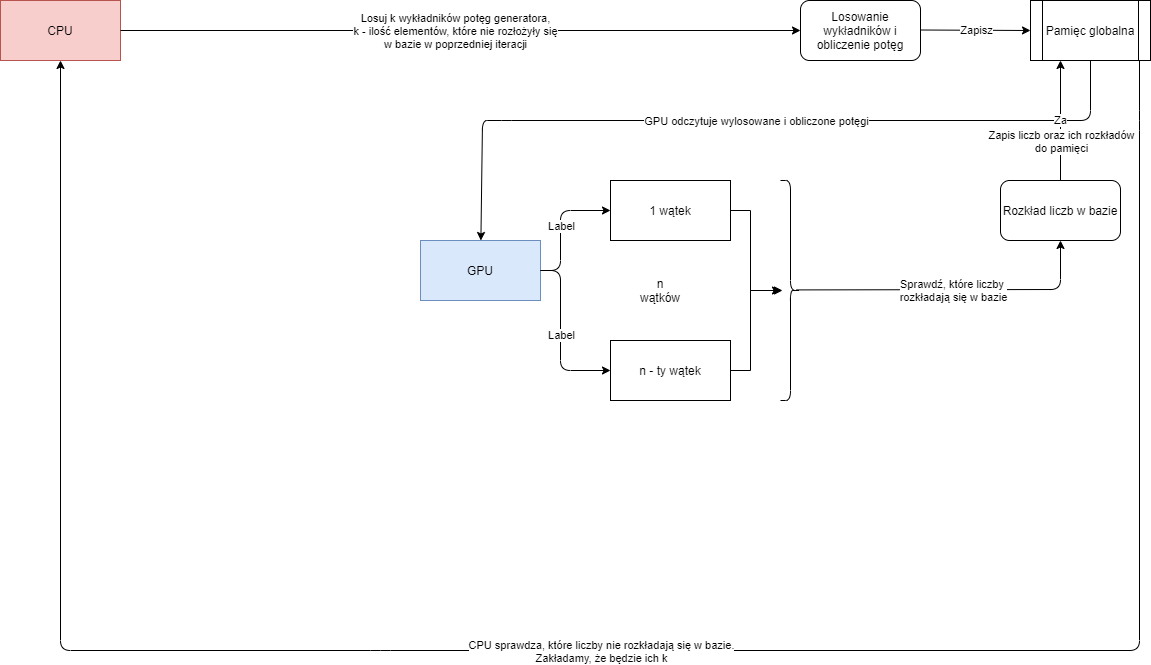
\includegraphics[width = 15 cm]{Diagram_uzupełnienie_do_n — kopia.png}
    \end{center}
    \newpage
    \item CPU sprawdza czy zbudowany układ równań jest oznaczony, jeśli tak to jest on rozwiązywany przy pomocy GPU. Jeśli układ nie jest oznaczony to CPU losuje kolejny wykładnik potęgi, sprawdza czy potęga rozkłada się w bazie i przekazuje układ na GPU, które rozwiązuje go metodą eliminacji Gaussa.\\
    Proces ten przedstawia poniższy diagram przepływu danych.
    \begin{center}
    \includegraphics[width = 15 cm]{Diagram_dodawanie-relacji — kopia.png}
    \end{center}
\end{enumerate}



\newpage

\section{Metoda indeksu}
Metoda indeksu jest najszybszym algorytmem rozwiązujacym problem logarytmu dyskretnego.\\
Zapewnia nam podwykładniczą złożoność rozwiązywania logarytmu.\\
Chcąc rozwiązać równanie $x=log_ab$ w grupie $F_p^*$,\\
gdzie $F_p^* = <a>$ rzędu p - 1. Zakładając, że rozwiązanie opisywanego problemu istnieje powinniśmy skorzystać z poniżej przedstawionego algorytmu.
\begin{enumerate}
    \item  Wyznaczamy zbiór pierwszych liczb B-gładkich (parametr B powinniśmy przyjmować indywidualnie dla każdego przypadku użycia algorytmu oddzielnie).
    \item Kolejnym krokiem jest konstrukcja zbioru relacji
    \begin{center}
        R = $\{a^{e_i}(mod$ p)$| a^{e_i} =  \prod_{j = 1}^{k} p_j^{a_{i,j}}, p_j \in N, i = 1, .. ,l\} $,\\
    \end{center}
    gdzie $l >= k$, dla wybranych $e_i$. Jest to l-elementowy zbiór takich $a_{e_i} \in F_p^*$, które rozkładają się w bazie N.
    \item Kolejnym krokiem jest skonstruowanie odpowiedniego układu równań stworzonego dzięki zbiorowi relacji, sprawdzenie przy pomocy twierdzenia Cronnecera-Cappeliego czy układ jest oznaczony, jeśli tak to rozwiązanie go, w przeciwnym przypadku powinniśmy wrócić do punktu nr 2.
    \item Następnie powinniśmy wylosować liczbę $r \in \{2, ..., p-2\}$, takie że $ba^r$(mod p) rozkłada się w bazie N. 
    \begin{center}
        $ba^r$(mod p) = $\prod_{j = 1}^{k} p_j^{r^j}$
    \end{center}
    dla pewnych $r_j \in N$
    \item Pozostaje nam obliczenie rozwiązania z poniższego wzoru\\
    \begin{center}
        $x \equiv -r + \sum_{j=1}^{k} r_jx_j$(mod n).
    \end{center}
\end{enumerate}
 
 \subsection{Pseudokod omówionej metody indeksu}
\begin{algorithm}[H]
\renewcommand{\algorithmicrequire}{\textbf{Wejście:}}
\renewcommand{\algorithmicensure}{\textbf{Wyjście:}}
\begin{algorithmic}[1]
    \REQUIRE $a, b, p, B$
    \ENSURE  $x$
    \STATE smooth = []
    \STATE r = 1
    \FOR{i in range(0, B)}
    \IF{licza i pierwsza}
    \STATE smooth += [i]
    \ENDIF
    \ENDFOR
    \STATE Skorzystaj z algorytmu tworzenai relacji, zbuduj zbiór R oraz odpowiedni układ równań $Ax = b$
    \STATE Rozwiąż układ równań, przechowaj jego rozwiązane w \textbf{x}
    \WHILE{True}
        \STATE r = randint(2, p-2)
        \IF{$ra^b$(mod p) rozkłada się w bazie}
        \STATE Przerwij wykonywanie pętli
        \ENDIF
    \ENDWHILE
    \STATE x = -r
    \FOR{i in range(0, k)} 
    \STATE x += $r_ix_i$(mod n) \# k to ilość elementów w zbiorze relacji
    \ENDFOR
\RETURN{x}
\end{algorithmic}
\end{algorithm}

\end{document}